\documentclass{article}
\usepackage{fullpage}
\usepackage{txfonts}
\usepackage{pgfplots}
\usepackage{siunitx}
\usepackage{graphicx}
\setcounter{secnumdepth}{0}

\newcommand\Ion[2]{\ensuremath{\mathrm{#1\,\scriptstyle #2}}}
\newcounter{ionstage}
\newcommand{\ion}[2]{% replace the aastex version
  \setcounter{ionstage}{#2}%
  \Ion{#1}{\Roman{ionstage}}}

% \usepgfplotslibrary{external}
% \tikzset{external/force remake}
% \tikzexternalize

\pgfplotsset{
  compat=1.5.1, % most current version as of writing (27 Jan 2012)
  % compat=newest, % select to always use latest version (may cause minor appearance changes)
  width=\textwidth,
  every axis legend/.append style={
    % make legend less tightly packed
    inner xsep=0.5em,
    inner ysep=3pt,
    nodes={
      inner xsep=1em,
      text depth=0.25em
    },
  },
}
\pgfplotsset{}
\newcommand\RatioPlot[1]{
\begin{tikzpicture}
  \begin{loglogaxis}[
    xlabel={Observed Intensity, \(100 \times I(\lambda)/I(\mathrm{H}\beta)\)}, 
    ylabel={Model Intensity, \(100 \times I(\lambda)/I(\mathrm{H}\beta)\)},
    log ticks with fixed point,
    legend columns=3,
    legend pos=north west,
    % transpose legend,
    ]
    \addplot [
    scatter/classes={
      H1={mark=*,brown},% 
      He1={mark=*,green},% 
      C2={mark=triangle*,black},%  
      N2={mark=triangle*,cyan},% 
      O1={mark=*,orange},% 
      O3={mark=square*,orange},%
      Ne3={mark=square*,blue},%
      S2={mark=triangle*,red},% 
      S3={mark=square*,red},% 
      Ar3={mark=square*,magenta},%
      Fe3={mark=square*,yellow}%
    },
    only marks, scatter, 
    scatter src=explicit symbolic,
    point meta=explicit symbolic,
    nodes near coords*={\scriptsize\pgfmathprintnumber[set thousands separator={}]\LAMBDA\,\AA},
    visualization depends on={\thisrow{Lambda} \as \LAMBDA},
    nodes near coords align=\ALIGN,
    visualization depends on={value\thisrow{Align} \as \ALIGN},    
    error bars/x dir=both,
    error bars/x explicit,
    error bars/y dir=none,
    ] table [
    x=Obs, 
    y=Model#1, 
    x error=Sigma,
    meta=ID
    ] {ratios-177341.dat};
    \addlegendentry{\ion{H}{1}} 
    \addlegendentry{\ion{He}{1}} 
    \addlegendentry{\ion{C}{2}} 
    \addlegendentry{[\ion{N}{2}]} 
    \addlegendentry{[\ion{O}{1}]}
    \addlegendentry{[\ion{O}{3}]}
    \addlegendentry{[\ion{Ne}{3}]}
    \addlegendentry{[\ion{S}{2}]}
    \addlegendentry{[\ion{S}{3}]}
    \addlegendentry{[\ion{Ar}{3}]}
    \addlegendentry{[\ion{Fe}{3}]}
    \addplot [gray,domain=0.08:300] {x};
  \end{loglogaxis}
\end{tikzpicture}
}

\begin{document} 


\section{Model A: Baseline model}
\begin{description}
\item[Spectrum] WMBasic, \SI{39000}{K}
\item[Flux] \(\log_{10} \Phi = 13.50\)
\item[Abundance set] Cloudy Orion
\end{description}
\bigskip
\RatioPlot{A}

\begin{itemize}
\item Significant disagreement with observations
\item Low ionization lines are too weak; high ionization lines are too strong
\item Iron lines are far too strong -- presumably due to abundance
\item Same for Argon line
\end{itemize}
\newpage 

\section{Model B: Lower flux}
\begin{description}
\item[Spectrum] WMBasic, \SI{39000}{K}
\item[Flux] \(\log_{10} \Phi = 13.20\)
\item[Abundance set] Cloudy Orion
\end{description}
\bigskip
\RatioPlot{B}

\begin{itemize}
\item Much better agreement, but still some differences
\item {}[\ion{O}{1}] is 30\% (0.11 dex) too weak; [\ion{O}{3}] nebular lines are 30\% too strong (but auroral line is OK)
\item {}[\ion{N}{2}], [\ion{S}{2}], and [\ion{S}{3}] are all marginally too weak by 10--20\%
\item Iron and Argon are the same as in A
\end{itemize}
\newpage 

\section{Model C:  Esteban abundances}
\begin{description}
\item[Spectrum] WMBasic, \SI{39000}{K}
\item[Flux] \(\log_{10} \Phi = 13.50\)
\item[Abundance set] Esteban et al.\@ (2004), M42, \(t^2 = 0.002\)
\end{description}
\bigskip
\RatioPlot{C}

\begin{itemize}
\item Slightly better than A in some respects, but worse in others
\item {}[\ion{Fe}{2}] is now much better, but Argon and Neon are worse because the abundance went up
\item {}[\ion{O}{3}] still has the nebular lines too strong, but now the auroral line is too weak as well.  The temperature in the high-ionization zones is obviously too low
\item Nitrogen is now too weak, and sulphur too strong, which can be directly ascribed to the changed abundances
\end{itemize}
\newpage 

\section{Model D: Tsamis abundances}
\begin{description}
\item[Spectrum] WMBasic, \SI{39000}{K}
\item[Flux] \(\log_{10} \Phi = 13.50\)
\item[Abundance set] Tsamis et al.\@ (2011), LV2
\end{description}
\bigskip
\RatioPlot{D}

\begin{itemize}
\item This is all over the place.  These abundances can definitely be ruled out.
\item Iron, Sulphur, and Nitrogen are too weak
\item Carbon is too strong, due to increased abundance
\item However, Argon is much improved, as is [\ion{O}{1}]
\item The [\ion{O}{3}] auroral/nebular ratio is still too small
\end{itemize}
\newpage  

\section{Model E: Tlusty atmosphere}
\begin{description}
\item[Spectrum] Tlusty, \SI{39000}{K}
\item[Flux] \(\log_{10} \Phi = 13.50\)
\item[Abundance set] Cloudy Orion
\end{description}
\bigskip
\RatioPlot{E}

\begin{itemize}
\item 
\end{itemize}
\newpage 

\section{Model F: Lower flux and Esteban}
\begin{description}
\item[Spectrum] WMBasic, \SI{39000}{K}
\item[Flux] \(\log_{10} \Phi = 13.20\)
\item[Abundance set] Esteban et al.\@ (2004), M42, \(t^2 = 0.002\)
\end{description}
\bigskip
\RatioPlot{F}
\newpage 

\section{Model G: Intermediate flux and Esteban}
\begin{description}
\item[Spectrum] WMBasic, \SI{39000}{K}
\item[Flux] \(\log_{10} \Phi = 13.35\)
\item[Abundance set] Esteban et al.\@ (2004), M42, \(t^2 = 0.002\)
\end{description}
\bigskip
\RatioPlot{G}
\newpage


\section{Model H: Cooler star}
\begin{description}
\item[Spectrum] WMBasic, \SI{38000}{K}
\item[Flux] \(\log_{10} \Phi = 13.50\)
\item[Abundance set] Cloudy Orion
\end{description}
\bigskip
\RatioPlot{H}
\clearpage

\section{Model I: Bespoke abundances and lower flux}
\begin{description}
\item[Spectrum] WMBasic, \SI{39000}{K}
\item[Flux] \(\log_{10} \Phi = 13.20\)
\item[Abundance set] Tweak01
\end{description}
\bigskip
\RatioPlot{I}

\begin{itemize}
\item This is the best one!  Nearly everything is OK, except\dots
\item \dots the nebular [\ion{O}{3}] lines are 20--30\% too strong (about \(3 \sigma\))
\item \dots and [\ion{O}{1}] is too weak, but that does not matter, since there will be a contribution from OH dissociation in the neutral disk wind, which is not include in the model
\end{itemize}

\clearpage

\section{Model J: Bespoke abundances (50\% Oxygen) and lower flux}
\begin{description}
\item[Spectrum] WMBasic, \SI{39000}{K}
\item[Flux] \(\log_{10} \Phi = 13.20\)
\item[Abundance set] Tweak02
\end{description}
\bigskip
\RatioPlot{J}

\clearpage
\section{Model K: Further tweaked abundances (50\% Oxygen) and lower flux}
\begin{description}
\item[Spectrum] WMBasic, \SI{39000}{K}
\item[Flux] \(\log_{10} \Phi = 13.20\)
\item[Abundance set] Tweak03
\end{description}
\bigskip
\RatioPlot{K}

\clearpage

\newlength\figwidth
\setlength\figwidth{0.3\linewidth}
\setkeys{Gin}{width=\linewidth}
\newcommand\NTfig[2]{%
  Model #1 -- \texttt{#2}\par\medskip
  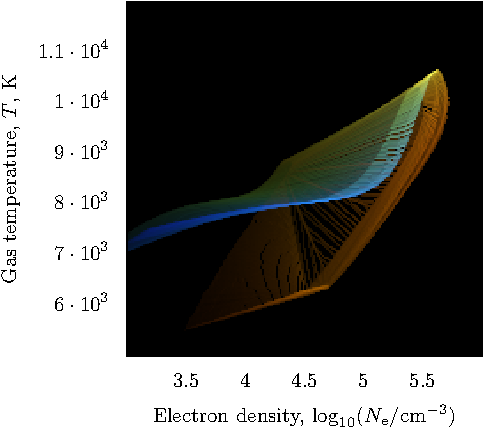
\includegraphics{../models/proplyd-auto-models/#2/NT-plane-ONO}
}
\renewcommand\arraystretch{2.5}\scriptsize
\begin{tabular*}{\linewidth}{
    @{\extracolsep{\fill}}
    p{\figwidth} 
    p{\figwidth} 
    p{\figwidth} 
  }
  \NTfig{A}{WM039000-phi13.50-r15.28} & 
  \NTfig{B}{WM039000-phi13.20-r15.28} & 
  \NTfig{C}{WM039000-phi13.50-r15.28-ZE} \\ 
  \NTfig{D}{WM039000-phi13.50-r15.28-ZT} & 
  \NTfig{E}{TL039000-phi13.50-r15.28} & 
  \NTfig{F}{WM039000-phi13.20-r15.28-ZE} \\ 
  \NTfig{G}{WM039000-phi13.35-r15.28-ZE} & 
  \NTfig{H}{WM038000-phi13.50-r15.28} & 
  \NTfig{I}{WM039000-phi13.20-r15.28-ZZ} \\ 
  \NTfig{J}{WM039000-phi13.20-r15.28-ZZ02} & 
  \NTfig{K}{WM039000-phi13.20-r15.28-ZZ03} & 
\end{tabular*}


% The marker for [\ion{Ne}{3}] is \ref{marker:Ne3}

\end{document}
